\documentclass[11pt]{article}

\usepackage[utf8]{inputenc}
\usepackage[a4paper,margin=2.4cm]{geometry}
\usepackage{amsmath,amssymb}
\usepackage{graphicx}
\usepackage{booktabs}
\usepackage{siunitx}
\usepackage{longtable}
\usepackage{caption}
\usepackage[section]{placeins}
\usepackage{parskip}
\usepackage{xcolor}
\usepackage{todonotes}
\definecolor{citegreen}{rgb}{0.0,0.45,0.0}
\usepackage[colorlinks=true,citecolor=citegreen,linkcolor=black,urlcolor=citegreen]{hyperref}

\graphicspath{{figures/}}
\captionsetup{font=small,labelfont=bf}
\sisetup{detect-all}
\renewcommand{\arraystretch}{1.15}

\title{\textbf{Reinforcement Learning Guidance for Re-entry}}
\author{\'Alvaro Carrasco Tabera}
\date{\today}

\begin{document}
\maketitle

\section{Introduction}

The successive convexification guidance developed for this vehicle solves a constrained trajectory optimization problem online, at every guidance call, and enforces the path and terminal constraints explicitly. It is accurate and robust, but it comes with the cost of an onboard convex solver, a runtime per call of several seconds and a strong dependence on the quality of the warm start and of the penalty weights. A guidance law that links the current state directly to a command, without solving an optimization problem in the loop, is attractive as a complement to it. This is the role investigated here for a policy trained by reinforcement learning.

The motivation is based on three different points. First, the execution cost of a trained network is a fixed sequence of matrix products, well under a millisecond on modest hardware and constant from call to call, against the several seconds and the convergence dependent variability of the online solver. Second, the policy is a feedback map from the state and therefore reacts to the actual flown condition by construction, with no reference trajectory to store or to re-time and no dependence on an initial guess. Third, the onboard software reduces to the evaluation of a fixed network, removing the convex solver and its numerical failure modes from the flight critical path. As a downside, the learned policy offers no guarantee of constraint satisfaction and, in the form studied here, controls only the terminal position and not the full terminal state including the velocity vector. The purpose of this work is to establish what such a policy can achieve on the reference mission and to document the development that took it there, so that the trade can be judged on measured results.

The remainder of the report is organized as follows. Section~\ref{sec:fd} establishes the flight dynamics core that serves as the training environment and validates it against the successive convexification generated command profile. Section~\ref{sec:env} defines the reinforcement learning environment and the baseline learning algorithm. Section~\ref{sec:campaign} documents the reward shaping campaign, including the reward formulation and its evolution, and reports the full set of versions. Section~\ref{sec:hpo} reports the hyperparameter optimization. Section~\ref{sec:conclusion} concludes.

\section{Flight Dynamics Core}
\label{sec:fd}

The environment integrates a three degree of freedom translational point mass model on a rotating oblate Earth, identical in its physics to the guidance model of the successive convexification framework, so that a policy trained here can be compared against that reference on equal terms. The model is a faithful port of the reference simulator and its agreement with it is quantified at the end of this section.

\subsection{Equations of Motion}

The translational motion is described in rotating planet fixed spherical coordinates by the geocentric radius $r$, the longitude $\lambda$, the latitude $\delta$, the Earth relative speed $V$, the flight path angle $\gamma$ and the heading $\psi$. It is governed by the three degree of freedom equations of motion on a rotating oblate Earth, with the gravitational acceleration retaining the central term and the second zonal harmonic $J_2$, because a re-entry spans many minutes and the terminal accuracy required for a precision handover is sensitive to the oblateness term. The full equations are standard and are given in the re-entry dynamics literature~\cite{mooij1994motion,mooij2024reentrysystems,dominguez2021abort}; they are not reproduced here.

The bank angle and the angle of attack are appended to the state and driven by the commanded rates $\dot\sigma=u_\sigma$ and $\dot\alpha=u_\alpha$, so that the policy commands rates rather than angles. Commanding rates produces smooth attitude histories, lets the actuator rate limits act as simple bounds on the action and presents the attitude loop with easier magnitudes it can track. The integration is carried out in a non dimensional form scaled by the reference Earth radius and circular orbital speed, with a fourth order Runge Kutta scheme and three substeps per one second guidance interval.

\subsection{Environment and Vehicle Models}

The atmosphere is the U.S.\ Standard Atmosphere of 1976, a layered model on geopotential altitude extended above its tabulated range by an isothermal exponential whose scale height is evaluated at the boundary temperature, which keeps the density and its altitude derivative continuous across the handover~\cite{ussa1976}. The altitude fed to the atmosphere is measured above the local WGS-84 ellipsoid radius, so every atmospheric quantity acquires a latitude dependence. Only the density and the speed of sound are required by the force and constraint models.

The reference vehicle is the WB001 winged body. Its lift and drag coefficients are polynomial functions of the angle of attack, and the lift and drag follow $L=\tfrac12\rho V^2 S_{\mathrm{ref}}C_L$ and $D=\tfrac12\rho V^2 S_{\mathrm{ref}}C_D$ with reference area $S_{\mathrm{ref}}=\SI{391.22}{\meter\squared}$ and mass $m=\SI{104305}{\kilo\gram}$. The stagnation point heat rate is the Sutton--Graves power law $\dot Q=k_Q\,\rho^{0.5}V^{3.15}$ with $k_Q=\SI{1.65e-4}{}$ in SI base units~\cite{suttongraves1971}. Three path constraints bound the flight, on the heat rate, the load factor $n=\sqrt{L^2+D^2}/(mg_0)$ and the dynamic pressure $\bar q=\tfrac12\rho V^2$. The mission and the path constraint limits are collected in Table~\ref{tab:mission}.

\begin{table}[t]
\centering
\caption{Reference mission and path constraints for the WB001 vehicle. The initial and target states define a great circle range of \SI{7843}{\kilo\meter}.}
\label{tab:mission}
\begin{tabular}{@{}lll@{}}
\toprule
\textbf{Quantity} & \textbf{Entry interface} & \textbf{Target handover} \\
\midrule
Altitude              & \SI{100}{\kilo\meter} & \SI{25}{\kilo\meter} \\
Longitude, latitude   & \ang{0}, \ang{0}      & \ang{12}, \ang{70} \\
Earth relative speed  & \SI{7450}{\meter\per\second} & free \\
Flight path angle     & \ang{-0.5}            & \ang{-10} (not enforced by the policy) \\
Heading               & \ang{0}               & \ang{90} (not enforced by the policy) \\
\midrule
\textbf{Path constraint limit} & \multicolumn{2}{l}{$\dot Q_{\max}=\SI{1.5}{\mega\watt\per\meter\squared}$,\quad $n_{\max}=2.5\,g_0$,\quad $\bar q_{\max}=\SI{18}{\kilo\pascal}$} \\
\textbf{Control rate limit} & \multicolumn{2}{l}{$|\dot\sigma|\le\ang{45}/\text{s}$,\quad $|\dot\alpha|\le\ang{15}/\text{s}$} \\
\bottomrule
\end{tabular}
\end{table}

\subsection{Validation}
\label{sec:validation}

The flight dynamics core is validated by prescribing the optimal bank and angle of attack command history of the successive convexification minimum heat load solution through the equations of motion, integrating from the reference initial condition and comparing the resulting trajectory node for node against the reference simulator. Figure~\ref{fig:validation} shows the absolute residual of the altitude, latitude, longitude and speed against time. The residuals grow slowly and monotonically along the trajectory, as expected from the accumulation of small integration differences, and remain bounded by \SI{20}{\meter} in altitude and \SI{0.9}{\meter\per\second} in speed at the terminal node after a flight of over \SI{1500}{\second}. The integrated heat load matches the reference to \SI{0.0004}{\percent}. This agreement confirms that a policy trained in this environment is optimizing against the same physics as the reference guidance.

\begin{figure}[ht]
\centering
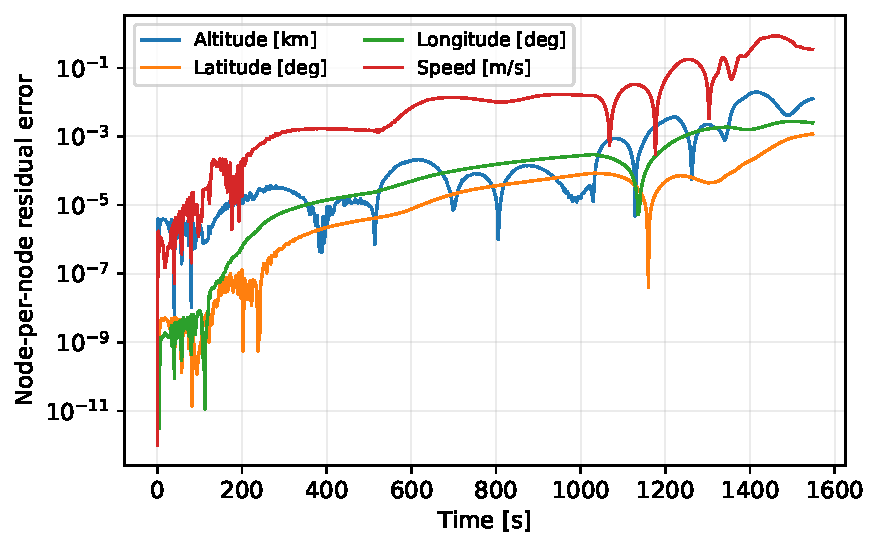
\includegraphics[width=0.72\linewidth]{validation_residual.pdf}
\caption{Node-per-node residual of the flight dynamics core against the successive convexification reference, with the reference command profile replayed through the equations of motion. The terminal residuals are \SI{20}{\meter} in altitude and \SI{0.9}{\meter\per\second} in speed.}
\label{fig:validation}
\end{figure}

\section{Reinforcement Learning Environment}
\label{sec:env}

\subsection{Markov Decision Process}

The guidance task is set up as an episodic Markov decision process. The environment integrates the eight dimensional state $[r,\lambda,\delta,V,\gamma,\psi,\sigma,\alpha]$ over a fixed one second interval per step, and an episode terminates when the vehicle reaches the target altitude of \SI{25}{\kilo\meter}, or fails by skipping out above \SI{120}{\kilo\meter}, falling below the minimum speed or exceeding a flight path angle bound, or times out. An episode is scored a success when the terminal great circle position error is below \SI{1}{\kilo\meter}.

The action is the two dimensional vector of normalized bank and angle of attack rate commands in $[-1,1]^2$, scaled to the physical rate limits of Table~\ref{tab:mission}. The observation presented to the policy is a normalized feature vector built from the physical state: the altitude, the Earth relative speed, the flight path angle, the sine and cosine of the heading, the dynamic pressure, the Mach number, the heat flux, the load factor, the range to go as a fraction of the initial range, the heading error to the target, the current bank angle and the current angle of attack. This baseline observation is thirteen dimensional. A fourteenth feature, the base ten logarithm of the range to go, was added during the campaign for the reason given in Section~\ref{sec:campaign} and is present in all later versions. The observations are normalized online by a running mean and variance estimate.

\subsection{Reward Structure}
\label{sec:reward}

The reward is a sum of a dense per step term and a terminal term charged once at the end of the episode. Writing $d_t$ for the great circle range to go at step $t$ in kilometers, $\mathbf a_t$ for the action, $h_t$ for the altitude and $N$ for the episode length, the per step reward is
\begin{equation}
r_t = \underbrace{\Phi(d_{t-1}) - \Phi(d_t)}_{\text{potential shaping}}
      \;-\; w_p \min\!\Big(\textstyle\sum_{c} B(g_c),\, b_{\max}\Big)
      \;-\; w_e \lVert \mathbf a_t - \mathbf a_{t-1}\rVert^2 \,\text{ if } [h_t < h_e],
\label{eq:rstep}
\end{equation}
where $\Phi$ is a position potential developed in Section~\ref{sec:campaign}, the second term penalizes the path constraints through a soft barrier $B$ summed over the heat rate, load factor and dynamic pressure ratios $g_c=\{\dot Q/\dot Q_{\max},\,n/n_{\max},\,\bar q/\bar q_{\max}\}$ and capped at $b_{\max}$, and the third term is a low altitude smoothness guard active below $h_e$. The barrier is
\begin{equation}
B(g) = \Big(\frac{\max(0,\,g-g_s)}{1-g_s}\Big)^{2} + \max(0,\,g-1)\big(10 + 10\max(0,\,g-1)\big),
\label{eq:barrier}
\end{equation}
which is zero while the ratio $g$ stays below the soft threshold $g_s$, rises quadratically to unity at the limit and steeply beyond it. The potential shaping is potential based, so it telescopes over the episode to $\Phi(d_0)-\Phi(d_N)$ and therefore leaves the optimum unchanged while providing a gradient at every step.

The terminal reward, charged on every way the episode can end, is
\begin{equation}
r_T = -\Phi(d_N) \;-\; w_s \frac{1}{N}\sum_{t} \lVert \mathbf a_t - \mathbf a_{t-1}\rVert^{2}
      \;+\;
      \begin{cases}
      w_c\,\varrho(d_N), & \text{target reached (success)},\\[2pt]
      -\,w_f, & \text{failure or timeout},
      \end{cases}
\label{eq:rterm}
\end{equation}
with the first term the uniform position term, the second the episode mean action change and $\varrho$ the success bonus shape. In the final form of the reward the weights are $w_p=1$, $g_s=0.9$, $b_{\max}=3$, $w_e=1$ below $h_e=\SI{35}{\kilo\meter}$, $w_s=25$, $w_c=300$ and $w_f=50$. The functional forms of the potential $\Phi$ and the bonus $\varrho$, and the values of their parameters, are the object of the campaign and are given in Section~\ref{sec:campaign}.

\subsection{Learning Algorithm}

The policy is trained with Proximal Policy Optimization, an on policy actor critic method that improves the policy within a clipped trust region and estimates the advantage by generalized advantage estimation~\cite{schulman2017ppo,schulman2016gae}. The implementation is that of Stable-Baselines3 on a Gymnasium environment~\cite{raffin2021sb3,towers2024gymnasium}, with eight parallel environment workers and observation normalization. Both the actor and the critic are MLPs of two hidden layers of five hundred and twelve units. Each version is trained for ten million environment steps. The baseline hyperparameters, which are the starting point for the campaign of Section~\ref{sec:campaign} and the object of the optimization of Section~\ref{sec:hpo}, are collected in Table~\ref{tab:baseline}.

\begin{table}[t]
\centering
\caption{Baseline PPO configuration used through the reward shaping campaign.}
\label{tab:baseline}
\begin{tabular}{@{}llll@{}}
\toprule
\textbf{Parameter} & \textbf{Value} & \textbf{Parameter} & \textbf{Value} \\
\midrule
Network architecture     & $2\times512$ (actor and critic) & Discount $\gamma$        & 0.999 \\
Learning rate            & \num{3e-4} (linearly decayed)   & GAE $\lambda$            & 0.95 \\
Rollout length per env   & 2048                            & Clip range              & 0.2 \\
Minibatch size           & 512                             & Entropy coefficient     & \num{5e-3} \\
Epochs per update        & 10                              & Parallel workers        & 8 \\
\bottomrule
\end{tabular}
\end{table}

\section{Reward Shaping Campaign}
\label{sec:campaign}

The campaign is a sequence of nineteen training versions, each changing one aspect of the reward or the environment relative to the one before, with the terminal position error as the primary metric and path constraint feasibility as a hard requirement. This section describes the development in the order it happened, because each version was a response to the failure mode of the previous one, and the sequence is what produced the set of rules that made the reward robust. The complete set of versions is reported in Table~\ref{tab:campaign}.

\paragraph{Multi-term reward (v1--v6).} The first reward combined a heat load term, soft path constraint barriers, an action magnitude penalty, an action smoothness penalty, a low angle of attack floor, the dense position shaping and a terminal position and flight path angle term. It kept the trajectory feasible but stalled between \SI{130}{} and \SI{300}{\kilo\meter} of terminal error, and with so many weighted terms acting at once, the cause of the plateau could not be attributed to any one of them. This motivated simplifying the reward down to the position objective alone.

\paragraph{Exploit free terminal structure (v7--v9).} The reduced reward used the logarithmic position potential
\begin{equation}
\Phi(d) = w_o \log_{10}\!\max(d,1), \qquad w_o = 100,
\label{eq:phi_log}
\end{equation}
which evaluates as an equal cost per decade of range and provides a reasonable gradient from thousands of kilometers down to one. The way the terminal term was evaluated was crucial. When the terminal penalty was applied only on a successful landing, the policy learned to skip out and fail on purpose, because failing was cheaper than landing far from the target (v7). When the terminal penalty was removed and only the shaping was kept, the discount made ending the episode early more valuable than a long controlled glide, and the policy dived into the ground far downrange (v8). Charging the anchor $-\Phi(d_N)$ uniformly on every episode ending, as in Eq.~\eqref{eq:rterm}, removed both limit uses at once and produced a policy that closed on the target consistently (v9). The main outcome of this part of the campaign is that the terminal cost must be a function of the final position that is paid on every way the episode can end, so that no ending is preferred for its own sake.

\paragraph{Discount and per step penalties (v10--v11).} Raising the discount from $0.999$ to $0.9999$, so that the terminal reward was not attenuated over the long episode, brought the error down to \SI{43}{\kilo\meter} (v10). An attempt to reduce control chattering with a per step smoothness penalty of weight $0.05$ then brought the policy back to the diving behavior (v11). The reason is that a per step penalty on the action rate is, in expectation, a cost proportional to the episode length times the exploration noise variance, so it penalizes a long controlled glide far more heavily than a short dive, inverting the preference of both and choosing on the short dive. The rule is that a quantity to be minimized over a variable length episode must be charged as an episode mean evaluated at the termination, as the $w_s$ term of Eq.~\eqref{eq:rterm} does, not as an accumulated value per step.

\paragraph{Potential steepening and observation resolution (v12--v15).} Charging the smoothness as a terminal mean, together with the capped barrier of Eq.~\eqref{eq:barrier}, gave a clean reward that reached \SI{17.8}{\kilo\meter} (v12). Steepening the potential near the target with an additional decade cost inside \SI{50}{\kilo\meter}
\begin{equation}
\Phi(d) = w_o \log_{10} d + w_n \min\!\big(\log_{10} d,\ \log_{10} d_n\big), \qquad w_n = 300,\ d_n = \SI{50}{\kilo\meter},
\label{eq:phi_shelf}
\end{equation}
improved it to \SI{6.7}{\kilo\meter} (v13). Pushing the potential steeper still caused the policy to diverge rather than improve (v14). The cause was linked to the observation: the range to go was presented only as a fraction of the initial range, whose resolution at the kilometer scale is of order \num{e-4}, which is orders of magnitude below something the network can resolve. This implied that a steeper reward acted on the observed states that the policy could not distinguish. Adding the base ten logarithm of the range to go as an observation, which carries equal resolution per decade down to the target, removed the divergence (v15).

\paragraph{Reward curvature (v16--v19).}  The last group is related to the curvature of the terminal position reward and its effect on the exploration noise. Because the terminal return depends on $\Phi(d_N)$, the shape of $\Phi$ determines whether variability in the final landing position is rewarded or penalized. If $\Phi$ is convex, Jensen's inequality implies that the expected reward of a spread-out distribution of landing points is greater than the reward obtained at the mean landing position \cite{boyd2004convex}. In other words, even when the average landing point does not improve, the agent can obtain a higher expected return simply by maintaining a large amount of exploration noise, since a few exceptionally good landings outweigh many less precise ones. This behavior was observed with the logarithmic potential of Eq.~\eqref{eq:phi_log}, which is convex in $d$. Therefore, the stochastic training return remained consistently higher than the deterministic evaluation return and the policy never fully settled. Replacing the near field by a linear well, matched to the logarithmic shelves at the boundary,
\begin{equation}
\Phi(d) = w_\ell\, d \quad (d \le d_\ell), \qquad w_\ell = 40,\ d_\ell = \SI{10}{\kilo\meter},
\label{eq:phi_lin}
\end{equation}
is neutral to dispersion and gave the best result of the campaign at \SI{5.4}{\kilo\meter} (v16). A concave near field, obtained by a convex combination of the linear and quadratic forms,
\begin{equation}
\Phi(d) = w_\ell d_\ell\Big[(1-\kappa)\frac{d}{d_\ell} + \kappa\Big(\frac{d}{d_\ell}\Big)^{2}\Big] \quad (d \le d_\ell), \qquad \kappa = 0.5,
\label{eq:phi_convex}
\end{equation}
penalizes dispersion and was introduced together with a stronger, concave success bonus to drive the action noise down (v18, v19). It removed the training to evaluation gap but did not on its own break below the five kilometer level within the training budget. The success bonus shape $\varrho$ evolved in parallel, from an indicator on the one kilometer disk in the early versions, through a linear ramp $\varrho(d)=\max(0,\,1-d/d_r)$ with $d_r=\SI{5}{\kilo\meter}$ in v16, to the concave $\varrho(d)=\max(0,\,1-(d/d_r)^2)$ with $d_r=\SI{10}{\kilo\meter}$ and $w_c$ raised from $100$ to $500$ in v19, so that the bonus provides a dense gradient over the last kilometers rather than firing only on a rare lucky landing. A cold start with no warm start was also run in this group and confirmed that the constant angle of attack behavior of the trained policies is an consequence of the warm start rather than a limitation of the reward, but it diverged on position and did not reach the target (v17).

\begin{table}[t]
\centering
\caption{Reward shaping campaign. Each row re-evaluates the best checkpoint of one version deterministically in the flight dynamics core. The heat load column is the integrated heat load relative to the successive convexification minimum heat load reference of \SI{1.072e9}{\joule\per\meter\squared}. Feasibility is met when every path constraint ratio stays at or below unity, marginal when below \num{1.02}. The final row is the best policy after the hyperparameter optimization of Section~\ref{sec:hpo}.}
\label{tab:campaign}
\begin{tabular}{@{}llS[table-format=4.1]S[table-format=+2.1]l@{}}
\toprule
\textbf{Version} & \textbf{Principal change} & {\textbf{Error [\si{\kilo\meter}]}} & {\textbf{Heat load [\si{\percent}]}} & \textbf{Feasible} \\
\midrule
v1  & Multi-term reward (baseline)         & 268.5 & +30.1 & No \\
v2  & Aborted   & {--}  & {--}  & {--} \\
v3  & Low angle of attack floor term       & 139.3 & -7.2  & Yes \\
v4  & Position weight raised               & 128.2 & -5.8  & Yes \\
v5  & Repeat under a new seed              & 160.6 & -5.5  & Yes \\
v6  & Reduced smoothness, higher entropy   & 308.9 & -0.4  & Yes \\
v7  & Minimal position only reward         & {fail}& {--}  & No \\
v8  & Terminal reward removed              & 4238.0& +21.0 & No \\
v9  & Uniform terminal reward              & 256.1 & +33.4 & No \\
v10 & Discount raised to \num{0.9999}      & 43.5  & -4.9  & Marg. \\
v11 & Per-step smoothness penalty          & 634.4 & -10.8 & No \\
v12 & Terminal mean smoothness, capped barrier & 17.8 & -4.3 & Yes \\
v13 & Near-field potential steepened       & 6.7   & -4.5  & Yes \\
v14 & Inner shelf and burst guard          & 22.1  & -4.9  & Yes \\
v15 & Logarithmic range observation        & 17.0  & -2.6  & Yes \\
v16 & Linear dispersion neutral well     & 5.4   & -5.3  & Yes \\
v17 & Cold start                           & 130.6 & -7.8  & Yes \\
v18 & Concave precision well               & 25.8  & -4.2  & Yes \\
v19 & Precision polish, low action noise   & 7.9   & -4.7  & Yes \\
\midrule
HPO & Tuned algorithm hyperparameters      & 0.3   & -5.2  & Yes \\
\bottomrule
\end{tabular}
\end{table}

The best reward shaping policy is version v16. Its altitude velocity profile shown in Figure~\ref{fig:reward_altvel}, it flies close to the heat rate path constraint boundary through the first high speed arc and stays inside the path constraints throughout, closely following the shape of the successive convexification optimum, which would be the general behavior expected for this type of flight. Its attitude history shown in Figure~\ref{fig:reward_aoabank}, has a smooth bank angle profile, while the angle of attack is held at its upper limit for the whole flight, which corresponds to the maximum L/D and is a behavior obtained from the warm-starting that the cold start of version v17 showed is not imposed by the reward. The learning curve shown in Figure~\ref{fig:reward_learning}, show the difficulty that motivated the second phase of the work: the terminal error reaches the five kilometer level in the best evaluations but oscillates rather than settling, and the deterministic evaluation return does not converge, which is the signature of a policy still limited by its exploration noise rather than by the reward.

\begin{figure}[ht]
\centering
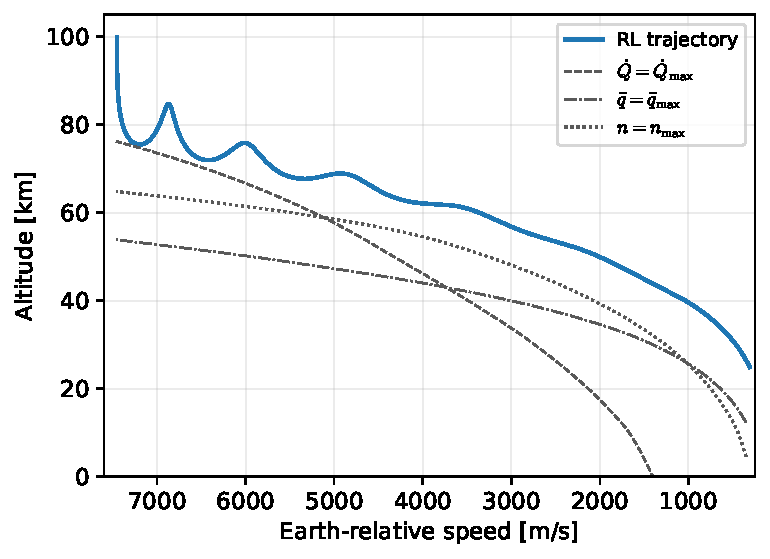
\includegraphics[width=0.60\linewidth]{reward_altvel.pdf}
\caption{Best reward shaping policy (v16): altitude against Earth relative speed.}
\label{fig:reward_altvel}
\end{figure}

\begin{figure}[ht]
\centering
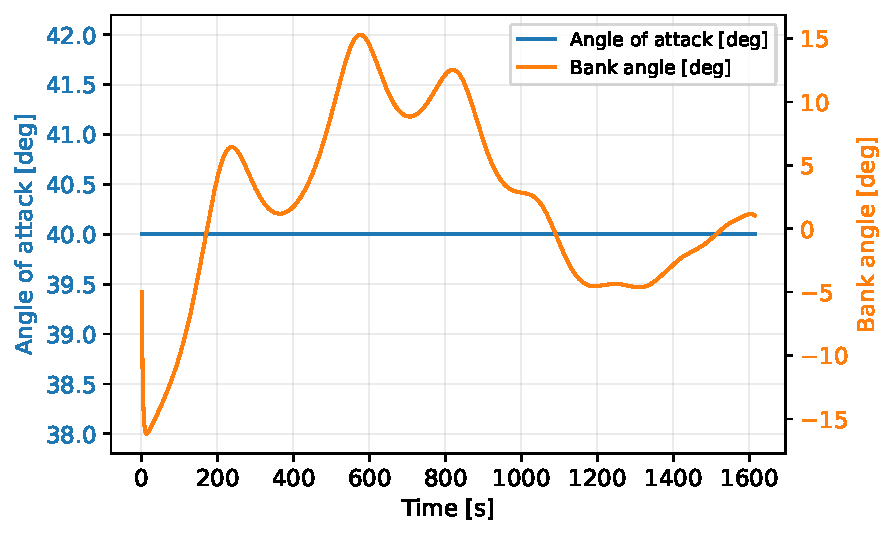
\includegraphics[width=0.62\linewidth]{reward_aoa_bank.pdf}
\caption{Best reward shaping policy (v16): angle of attack and bank angle against time.}
\label{fig:reward_aoabank}
\end{figure}

\begin{figure}[ht]
\centering
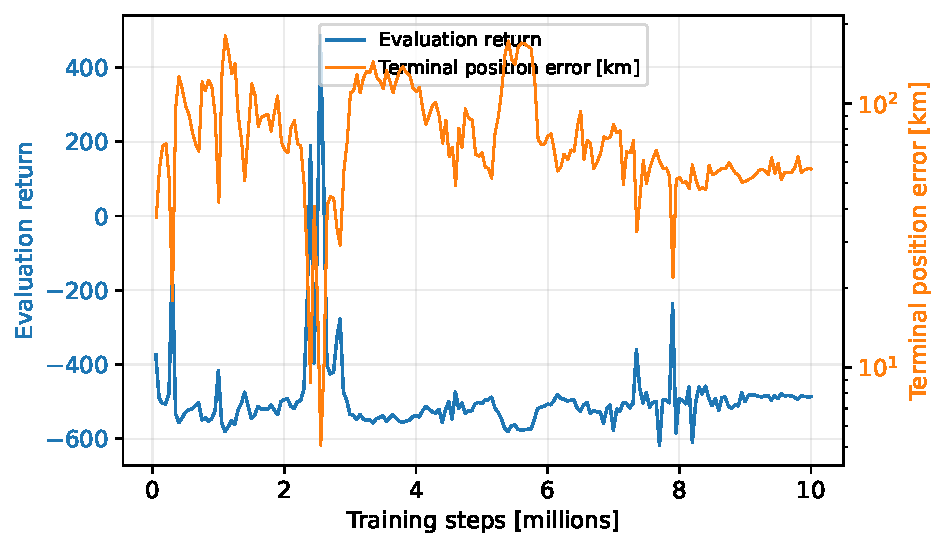
\includegraphics[width=0.66\linewidth]{reward_learning.pdf}
\caption{Training history of the best reward shaping version (v16): deterministic evaluation return and terminal position error against training steps.}
\label{fig:reward_learning}
\end{figure}

\section{Hyperparameter Optimization}
\label{sec:hpo}

The reward shaping campaign made clear that, from version v16 onward, the reward was adequate and the terminal error was limited by the learning dynamics rather than by the reward. Therefore, the next step was therefore to optimize the algorithm itself. This was done with an automatic study using the Optuna framework with a Tree structured Parzen Estimator sampler and a regulator that kills unpromising trials early~\cite{akiba2019optuna,bergstra2011tpe}.

\subsection{Strategy}

Every trial warm starts from the best reward shaping policy of version v16 and its observation normalization statistics, which fixes the network architecture and starts each trial from a feasible \SI{5.4}{\kilo\meter} solution rather than from scratch, so that the study measures the effect of the learning settings on a short polishing run of one and a half million steps rather than on a full training. The reward is frozen at the version v16 form for the whole study. Each trial is scored every hundred thousand steps by a deterministic evaluation, and the objective to be minimized is the best feasibility terminal error seen during the trial, where an infeasible evaluation is penalized so that the study never prefers an infeasible policy. Any policy that reaches a feasible error below six kilometers is saved immediately, because the best policies were found to occur between the periodic checkpoints. The search space is given in Table~\ref{tab:hpo_space}.

\begin{table}[t]
\centering
\caption{Hyperparameter search space.}
\label{tab:hpo_space}
\begin{tabular}{@{}lll@{}}
\toprule
\textbf{Hyperparameter} & \textbf{Range} & \textbf{Scale} \\
\midrule
Initial action standard deviation & \numrange{0.02}{0.3}       & logarithmic \\
Learning rate                      & \numrange{1e-5}{3e-4}      & logarithmic \\
Rollout length per environment     & $\{1024,2048,4096\}$       & categorical \\
Minibatch size                     & $\{256,512,1024,2048\}$    & categorical \\
Epochs per update                  & \numrange{3}{15}           & integer \\
Discount, as $1-\gamma$            & \numrange{5e-5}{2e-3}      & logarithmic \\
GAE $\lambda$                      & \numrange{0.90}{0.99}      & linear \\
Clip range                         & \numrange{0.05}{0.3}       & logarithmic \\
Entropy coefficient                & \numrange{1e-8}{5e-3}      & logarithmic \\
\bottomrule
\end{tabular}
\end{table}

\subsection{Result}

The study ran 41 trials, of which 11 completed and 29 were pruned early. The best trial reached a terminal error of \SI{0.27}{\kilo\meter}, inside the one kilometer success disk and inside the path constraints boundary, improving a factor of 20 over the best reward shaping policy obtained by tuning the learning algorithm alone. Figure~\ref{fig:hpo_history} shows the progress of the study. The relevant parameters reported by the study rank the minibatch size, the rollout length and the initial action standard deviation as the dominant factors, ahead of the learning rate, with the remaining hyperparameters of minor influence over the searched ranges. The reason for this is that the terminal precision is set mainly by how well the policy gradient is averaged, through the batch and rollout sizes and by how much exploration noise is kept in the deterministic policy, through the action standard deviation. The best configuration is given in Table~\ref{tab:hpo_best}, and the resulting trajectory is compared against the successive convexification reference in Section~\ref{sec:comparison}.

\begin{table}[t]
\centering
\caption{Best hyperparameter configuration found by the study.}
\label{tab:hpo_best}
\begin{tabular}{@{}llll@{}}
\toprule
\textbf{Parameter} & \textbf{Value} & \textbf{Parameter} & \textbf{Value} \\
\midrule
Initial action std & 0.021          & Discount $\gamma$    & 0.99965 \\
Learning rate      & \num{1.41e-4}  & GAE $\lambda$        & 0.908 \\
Rollout length     & 4096           & Clip range           & 0.079 \\
Minibatch size     & 256            & Entropy coefficient  & \num{3.6e-4} \\
Epochs per update  & 5              & &  \\
\bottomrule
\end{tabular}
\end{table}

\begin{figure}[ht]
\centering
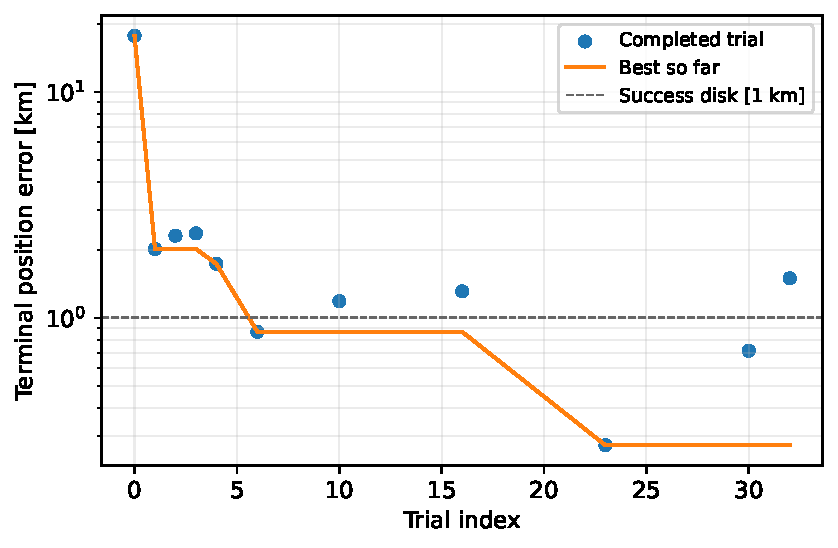
\includegraphics[width=0.66\linewidth]{hpo_history.pdf}
\caption{Progress of the hyperparameter study: the terminal error of each completed trial and the running best against the trial index.}
\label{fig:hpo_history}
\end{figure}

\subsection{Comparison and Limitations}
\label{sec:comparison}

The trajectory of the best learned policy is compared against the closed-loop successive convexification result on the same mission in Figures~\ref{fig:compare_altvel} and~\ref{fig:compare_controls}. In the altitude velocity plane, Figure~\ref{fig:compare_altvel}, the two trajectories are almost indistinguishable through the hypersonic arc, both riding the heat rate boundary, and separate only in the low speed terminal phase, so the learned policy recovers the trajectory shape of the optimizer from the reward signal alone. The control histories, Figure~\ref{fig:compare_controls}, show where the two differ. The successive convexification solution modulates the angle of attack, reducing it to about \ang{28} near the handover to manage the terminal energy, whereas the learned policy holds the angle of attack at its upper limit for the whole flight and steers with the bank angle alone. The learned policy therefore reaches the target position using a single control axis where the optimizer uses two, which is consistent with the constant angle of attack behavior noted throughout the campaign.

\begin{figure}[ht]
\centering
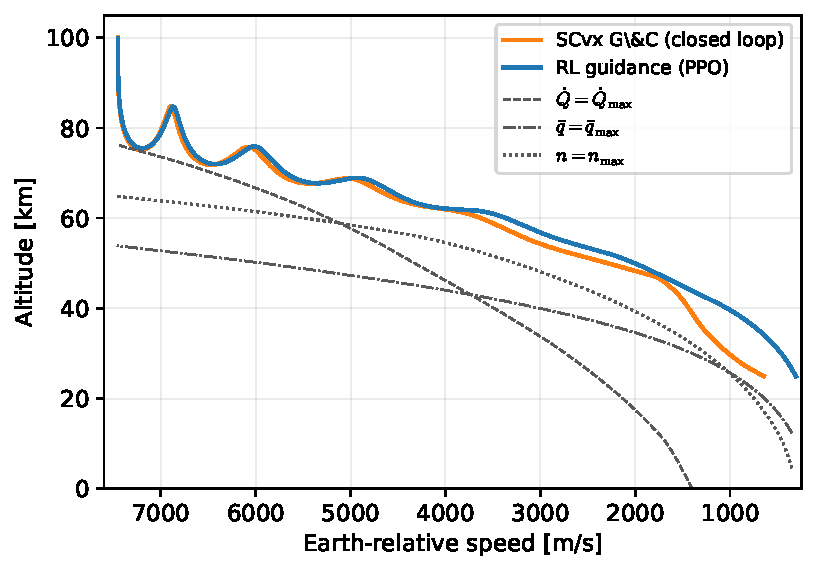
\includegraphics[width=0.62\linewidth]{compare_altvel.pdf}
\caption{Altitude against Earth relative speed for the best learned policy and the closed-loop successive convexification guidance and control result, with the path constraint boundaries. The two trajectories are almost indistinguishable through the hypersonic arc.}
\label{fig:compare_altvel}
\end{figure}

\begin{figure}[ht]
\centering
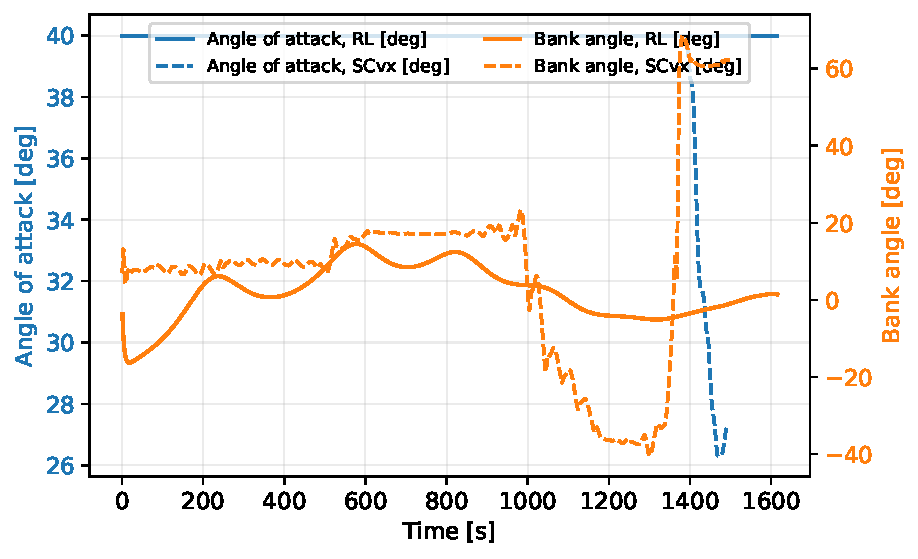
\includegraphics[width=0.64\linewidth]{compare_controls.pdf}
\caption{Angle of attack and bank angle against time for the best learned policy and the successive convexification reference. The optimizer modulates the angle of attack to about \ang{28} near the handover, while the learned policy holds it at its upper limit and steers with the bank angle alone.}
\label{fig:compare_controls}
\end{figure}

The best learned policy reaches the target to \SI{0.27}{\kilo\meter}, against the \SI{42}{\meter} of the closed-loop successive convexification guidance and control result on the same mission, at a per call inference cost of well under a millisecond against several seconds per solver call. However, there are two explicit limitations that should be mentioned. First, the learned policy controls the terminal position only and leaves the terminal flight path angle and heading uncontrolled, so it arrives at the handover altitude with a velocity orientation that the successive convexification solution fixes as part of its terminal constraints. Second, the successive convexification result is a full closed-loop guidance and control assessment, with a three axis attitude loop and its actuators in the loop and with explicit path and terminal constraint enforcement, whereas the present result is a three degree of freedom guidance policy with no formal constraint guarantee and an infinite bandwidth inner attitude loop. The learned policy recovers the trajectory shape and, after the hyperparameter optimization, the position accuracy of the optimizer, but it does so as a guidance layer that would still require an attitude loop and a constraint monitor to become a complete architecture.

\section{Conclusion and Future Work}
\label{sec:conclusion}

A reinforcement learning guidance policy for atmospheric re-entry was developed on a validated three degree of freedom flight dynamics core and trained with PPO. A reward shaping campaign reduced the terminal position error from several hundred kilometers to \SI{5.4}{\kilo\meter} inside the path constraints and, in doing so, produced a small set of remarkable rules: the terminal cost must be evaluated uniformly on every episode ending, magnitudes minimized over a variable length episode must be evaluated as the mean in the terminal step rather than per step, the observation must provide information at the scale the reward acts on and the curvature of the terminal reward controls whether the policy is rewarded for concentrating or for dispersing its landings. A subsequent hyperparameter optimization of the learning algorithm, warm started from the best reward shaping policy, reached \SI{0.27}{\kilo\meter} inside the success disk, and identified the batch and rollout sizes and the exploration noise as the dominant factors, which located the true limit on terminal precision in the learning dynamics rather than in the reward shape itself.

Some possible future work could come in three directions. The first is to add the terminal velocity orientation to the objective, so that the policy controls the flight path angle and the heading as the successive convexification solution does, which the constant angle of attack behavior of the current policies suggests is within reach once the pitch control axis is exploited. The second is to assess the policy under uncertainty, by training under dispersed initial and terminal conditions as well as model uncertainty for instance and by conducting a Monte Carlo to evaluate robustness as done in the successive convexification guidance and control architecture. The third is to couple the RL guidance to the attitude loop and the actuator models of the reference or by constructing a RL controller by itself, so that the learned guidance policy could be judged, as the successive convexification guidance was, on the full closed-loop rather than on the guidance model alone.

\appendix

\section{Repository Structure}
\label{sec:appendix}

The framework is organized as a single Python architecture, \texttt{reentry\_rl}, with the flight dynamics core, the environments, the training and optimization scripts, the validation against the reference simulator and the post-processing separated in the subdirectories. The tree below shows the complete directory. The \texttt{results/} directory holds one run directory per training version, all of identical layout, as well as the hyperparameter study. Only one representative run is shown rather than every one of them.

{\footnotesize
\begin{verbatim}
reentry_RL/
|-- pyproject.toml                   package metadata and dependencies
|-- ARCHITECTURE.md                  design notes
|-- reentry_rl/                      source package
|   |-- physics/                     flight dynamics core (Sec. 2)
|   |   |-- constants.py             Earth, vehicle and mission constants
|   |   |-- atmosphere.py            US 1976 standard atmosphere
|   |   |-- gravity_j2.py            central and J2 gravity
|   |   |-- geodesy.py               ellipsoidal altitude, great-circle range
|   |   |-- aero_wb001.py            WB001 aerodynamics, heat rate, AoA schedule
|   |   `-- eom_3dof.py              3-DOF equations of motion, RK4 step
|   |-- envs/                        Gymnasium environments
|   |   |-- entry_env_base.py        base env: observation, reward, termination
|   |   |-- rewards.py               reward weights and position potential (Sec. 3.2, 4)
|   |   |-- stage1_bank.py           Stage 1 (bank only)
|   |   `-- stage2_bank_aoa.py       Stage 2 (bank and angle of attack)
|   |-- training/                    training and optimization
|   |   |-- train_sb3.py             PPO training entry point (CLI)
|   |   |-- common.py                vector-env construction, rollout metrics
|   |   |-- expand_obs.py            observation-space warm-start surgery (v15)
|   |   |-- hpo_optuna.py            Optuna hyperparameter study (Sec. 5)
|   |   `-- smoke_train_stage1.py    quick training smoke test
|   |-- validation/                  physics validation
|   |   |-- benchmark_scp.py         load SCvx reference trajectories
|   |   `-- validate_physics.py      command replay, node-per-node residual (Sec. 2.3)
|   `-- postprocessing/              figures and diagnostics
|       |-- plots.py                 trajectory profile plots
|       |-- diagnose_run.py          learning curves and checkpoint rollouts
|       |-- fig_scvx_vs_rl.py        SCvx-vs-RL altitude-velocity figure
|       |-- make_report_figures.py   all figures in this report
|       `-- validate_plots.py        validation plotting
|-- report/                          this report
|   |-- main.tex
|   |-- report.bib
|   `-- figures/                     generated PDF figures
`-- results/                         training runs and the HPO study
    |-- stage2_vNN/                  one directory per version, each containing:
    |   |-- config.json              run configuration
    |   |-- best/best_model.zip      best checkpoint by evaluation
    |   |-- ckpt/                    periodic checkpoints (model and normalizer)
    |   |-- evaluations.npz          evaluation history
    |   |-- eval_trajectory.csv      final deterministic rollout
    |   |-- train_log.txt            captured training log
    |   `-- diag/                    diagnostic figures
    `-- stage2_polish_hpo/           hyperparameter study
        |-- study.db                 Optuna SQLite storage (all trials)
        `-- trialNNN_*.zip           saved sub-kilometer trial policies
\end{verbatim}
}

\bibliographystyle{plain}
\bibliography{report}

\end{document}
